\section*{Points de départ}

\subsection*{Analyse des besoins}
\subsubsection*{Introduction}
\paragraph{}
Le large succès de Wikipedia(qui est le 2éme site le plus visité sur internet) et le progrès des techniques d’extraction des données ont abouti à la naissance de la construction automatique  de larges base de connaissances comme DBpedia, YAGO, etc...
\subparagraph{}
Beaucoup de connaissances sont construites en se basant sur l’extraction automatique des faits relationnels dans un texte.
Malheureusement, les bases de connaissances convergent sur les faits statiques et ne donnent pas une grande importance à la dimension temporelle.
Malgré le fait que la majorité des faits évoluent avec le temps, ou n'est valide que dans une période temporelle précise.
Ainsi, nous remarquons que le temps a une dimension significatif dans ces bases de connaissances.
\subparagraph{}
Dans cette étude on veut extraire des faits temporels et des évènements depuis des information semi-structurées de Wikipedia et Wikidata ; et textuelles de Wikipedia.
\paragraph{}
La dimension temporelle est particulièrement importante dans les relations binaires comme isPresidentOf, isCEOof, isMarriedTo, on peut être mariée à plusieurs épouses mais dans des différents intervalles de temps mais “On ne prend pas compte des exceptions de mariage polygames ”.
\subparagraph{}
Une base de connaissances contenant plusieurs présidents des États-Unis ne peut être consistante que lorsqu’on ajoute une dimension temporelle à ces faits. De plus l’annotation temporelle aide à faire la distinction entre les faits courants et et les faits dépassés.
Par exemple le fait “Kennedy est le président des États-Unis” est correct, mais n'est plus valide.
Lorsqu’on attache une annotation temporelle à un fait comme celui là, il devient universellement valide.
\subsubsection*{Problématique}
\paragraph{}
Lorsqu’on parcourt DBpedia on trouve beaucoup de triplets qui décrivent des informations temporelles. Ces derniers sont généralement liées à un contexte événementiel précis.
\subparagraph{}
Il est plus difficile d’exploiter ces informations si elles ne possèdent pas une structure claire et lisible par la machine.
\newline
Il se trouve que des informations liées au même contexte temporel dans DBpedia sont exprimées de la manière suivante: 
\begin{figure}[H]
        \centering
                \centering
                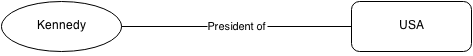
\includegraphics[width=10cm]{ken.png}
               \caption{triplet ''Kennedy''}

\end{figure}
\subparagraph{}
Le premier triplet n'a pas une sémantique valide que en tenant compte du triplet suivant~: 
\begin{figure}[H]
        \centering
                \centering
                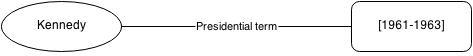
\includegraphics[width=10cm]{presidterm.png}
               \caption{triplet presidential term ''Kennedy''}

\end{figure}
\subparagraph{}
On vise plutôt à annoter les triplets (s,p,o) avec une étiquette temporelle qui précise la validité de ce terme dans un cadre logique qui appartient au monde réel où en dehors de ce cadre, on peut dire que ce triplet RDF n’est pas valide et qu’on ne peut pas l’utiliser.
\subsection*{Sources des données DBpedia}
\paragraph{}
Les faits temporels extraites de Wikipedia consiste en deux phases principales : extractions des données semi-structurées(tableaux, infoboxes) et l’extraction depuis le texte wikipédia.
\subsubsection*{Texte Wikipedia}
\paragraph{}
On cherche à extraire les informations temporelles qui ont un contexte de validité lié à un fait à partir des données textuelles des pages de Wikipedia. 
Par exemple sur la page de John Fitzgerald Kennedy, on retrouve~:
\newline
Kennedy a visité Berlin Ouest le 23 Juin 1963.
\subparagraph{}
On veut extraire les ressources en donnant une nouvelle structure pour mieux présenter leur contexte de validité temporelle.
\subsubsection*{Infobox Wikipedia}
\paragraph{}
Les infoboxes : Contiennent généralement les informations les plus importantes des entités décrites dans l’article. Par exemple dans l’infobox de “Kennedy” l’ancien président des États-Unis sur wikipédia on trouve la date d’élection, le prédécesseur du président, la durée du mandat, etc…
\newline
Chaque infoBox a un type particulier comme: évènement historique, élection, compétition ect…
\begin{figure}[H]
        \centering
                \centering
                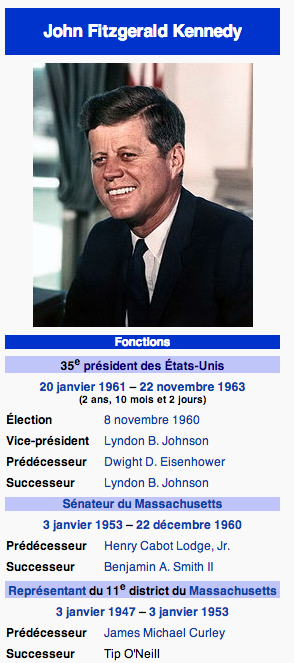
\includegraphics[width=5cm]{kennedy.png}
               \caption{Info Box Wikipedia ''Kennedy''}

\end{figure}
\subsubsection*{Tableau}
\paragraph{}
Dans les tableaux “Wikipedia” figurent des informations temporelles plus structurées et plus faciles à extraire, qu’on cherche à récupérer.
\subparagraph{}
Vous trouverez ci-dessous des informations sur les anciens précidents des États-Unis.
\begin{figure}[H]
        \centering
                \centering
                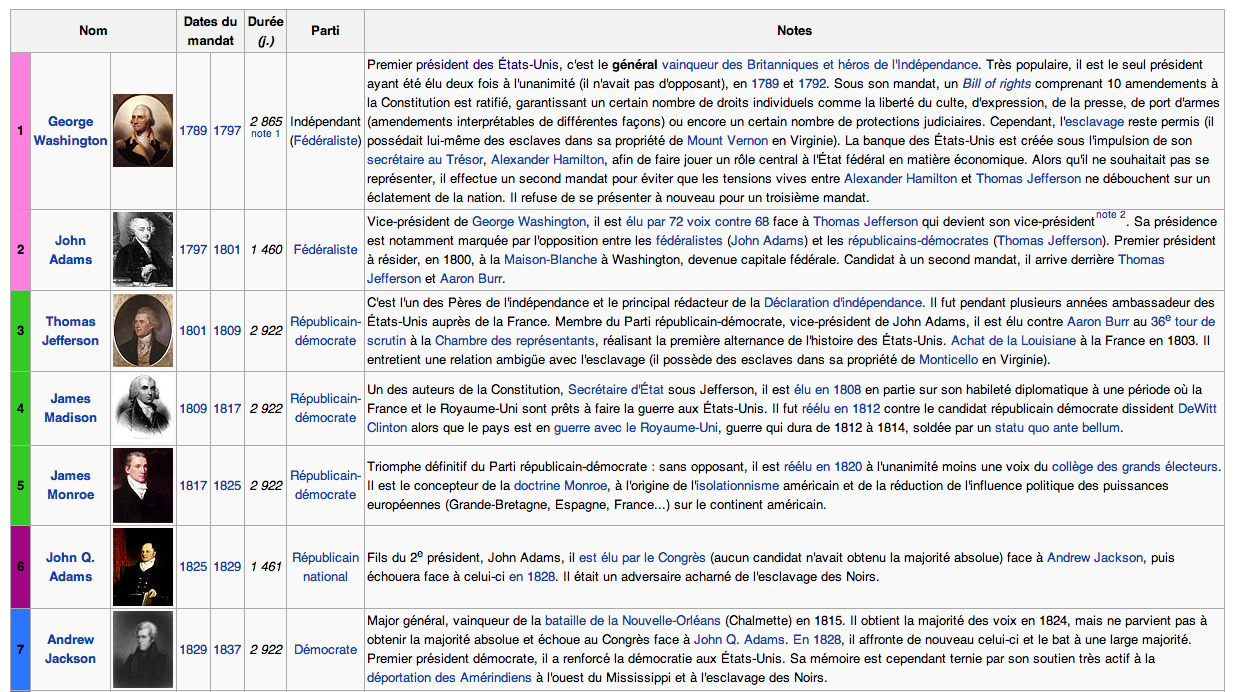
\includegraphics[width=14cm]{tableau.png}
               \caption{Exemple de tableau Wikipedia}

\end{figure}
\subsubsection*{Wikidata}
\paragraph{}
Sur la page wikidata, liée au contenu de la page wikipedia de Kennedy, on a intérêt à extraire les informations temporelles.
\begin{figure}[H]
        \centering
                \centering
                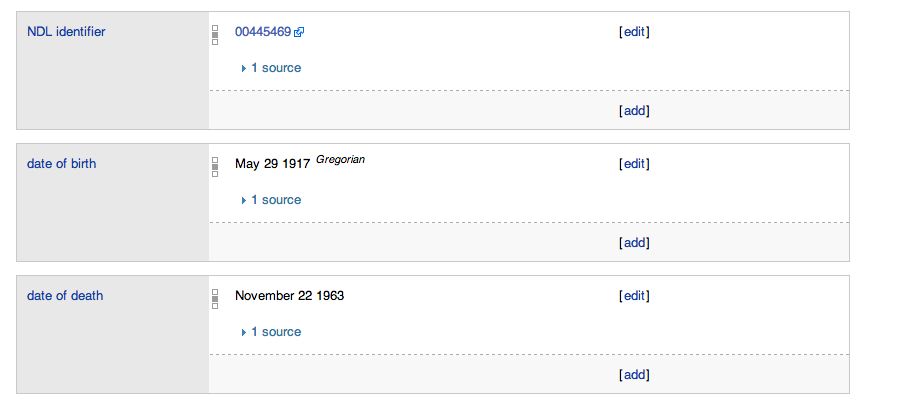
\includegraphics[width=14cm]{wikidata.png}
               \caption{Exemple Wikidata}

\end{figure}
\subsubsection*{Historique des pages wikipedia}
\paragraph{}
On souhaite, si c’est possible, extraire des informations temporelles relatives à l’historique de modifications des pages de wikipedia. Car, il se trouve qu’il y on a beaucoup d’informations liées à cet historique.
\subsubsection*{Résumé}
\paragraph{}
Il s'avère que beaucoup de points du temps dont liées à plusieurs sources d’information évènementielle; on cherche à extraire ces informations afin de les mettre sous une forme plus adéquate.
\subsection*{Notre modélisation}
\paragraph{}
Modèle quaternaire : un modèle qui capte la base du fait avec un indice temporel.
\newline
<politician> served as <politician office> from <date> to <date>
\newline
f1: Kennedy holdsPoliticalPosition PresidentOfUSA 
\newline
f2:f1 startedOnDate 
\newline
f3:f1 endedOnDate
\newline
HappenedDate est utilisée pour dire que le fait est valide que dans ce point du temps.
\begin{figure}[H]
        \centering
                \centering
                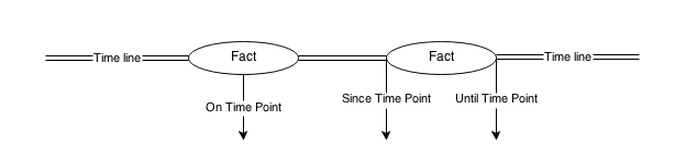
\includegraphics[width=10cm]{timeline.png}
               \caption{Event Time Line}

\end{figure}
\subparagraph{}
Pour surmonter ce problème et exprimer la validité temporelle d’un triplet RDF d’une manière à la fois intelligente et lisible par la machine; on souhaite rattacher au triplets valides que dans une plage temporelle bien précise une étiquette temporelle adéquate.
\newline
Exemple~:
\begin{figure}[H]
        \centering
                \centering
                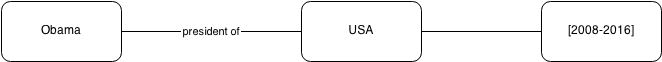
\includegraphics[width=10cm]{obamaQuad.png}
               \caption{Modélisation quadruplet}

\end{figure}
\subparagraph{}
On s'intéresse au format N-Quads qui est un standard w3c basé sur la forme N-Triples. L’avantage est qu’il se distingue par la possibilité d’encoder des graphes multiples.
Les quadruplets vont être formalisés de la manière suivante~:
\newline
$<s,p,o,[t1,t2]>$, un sujet, prédicat, objet avec une intervalle de temps.
\newline
$<s,p,o,t>$, de même avec un point de temps $t$.
\section*{Analyse temporelle}
\subsection*{Représentation}
\paragraph{}
Les informations temporelles peuvent avoir des repèsentations différentes~: 
\begin{itemize}
\item Un évènement `` Je vous propose un rendez-vous $demain$ pour parler de ma plateforme PiSharing``. \item Une connaissance `` Jacques Chirac est le président de la république Française `` \textbf{ mais quand ?}.
\end{itemize}
\subsection*{Ambiguïtés temporelles}
Le présent par exemple peut avoir plusieurs sens ou contextes : présent de narration, présent de généralité, présent qui réfère au futur proche, etc...
\subparagraph{}
Les signaux temporelles sont ambigus~: réunion de 14h à 16h, il court pour rattraper le temps, tu tournes après la rivière, etc…
\subparagraph{}
La plupart des expressions sont floues~: il y a deux ans, chaque deux semaines, j’arrive dans deux secondes, etc...
\paragraph{}
L’analyse du temps s’inscrit dans la compréhension globale des textes, et des évènements auxquels on fait référence dans ce texte. 
\newline
Modalité~: l’équipe de France voulait gagner la coupe du monde en 2006. 
\newline
Anaphore~: cela pourrait avoir lieu dans les éditions suivantes.
\subparagraph{}
Les évènements décrits (et que l’on souhaite fixer temporellement) peuvent être: duratifs ou ponctuels/accomplis ou inaccomplis. 
\subparagraph{}
De même pour les dates qui peuvent être~: Date absolue ``le 18 mars, c'est mon anniversaire``; Date relative par rapport au moment de l’énonciation~: `` il y a deux ans ``. Pour la durée~: Durée absolue `` durant 2 ans ``; Durée relative~: `` depuis un an ``.
\subparagraph{}
On trouve aussi~: Expression de fréquence `` tous les ans, le vendredi 13 ``, Expression plus complexe `` après la Révolution Tunisienne ``.
\subsection*{Résumé}
\paragraph{}
Dans l'encyclopédia libre Wikipedia, il se trouve qu’il y a beaucoup d’informations temporelles; qu'on risque de retrouver par la même occasion dans DBpedia. Dans cette étude on va plutôt essayer d’extraire des dates saillantes en fonction de leurs sémantiques évènementiels.